\documentclass[aspectratio=169]{beamer}

% ---------- ENCODING & FONTS ----------
\usepackage[utf8]{inputenc}
\usepackage[T1]{fontenc}

% ---------- THEME & LOOK ----------
\usetheme{Madrid}
\usecolortheme{seahorse}
\usefonttheme{professionalfonts}
\setbeamertemplate{navigation symbols}{}
\setbeamertemplate{footline}[frame number]
\setbeamercovered{transparent}
\setbeamertemplate{itemize items}[circle]
\setbeamertemplate{enumerate items}[default]
\setlength{\parskip}{0.25em}

% ---------- COLORS ----------
% Beamer loads xcolor; we just define colors.
\definecolor{accent}{RGB}{0,92,184}
\definecolor{soft}{RGB}{233,244,255}

\setbeamercolor{structure}{fg=accent}
\setbeamercolor{title}{fg=white,bg=accent}
\setbeamercolor{frametitle}{fg=accent}
\setbeamercolor{block title}{bg=accent!12,fg=accent}
\setbeamercolor{block body}{bg=soft}

% ---------- PACKAGES ----------
\usepackage{booktabs}
\usepackage{amsmath, amssymb}
\usepackage{array}
\usepackage{multirow}
\usepackage{hyperref}
\hypersetup{colorlinks=true,linkcolor=accent,urlcolor=accent}

% ---------- SAFE TRANSITION FALLBACK ----------
\makeatletter
\@ifundefined{transfade}{\newcommand{\transfade}[1][]{}}{}
\makeatother

% ---------- PLACEHOLDER BOX FOR FIGURES / TABLES ----------
\newcommand{\placeholderbox}[2][0.82\linewidth]{%
  \begin{center}
    \fbox{\begin{minipage}[c][0.46\textheight][c]{#1}
      \centering \vspace{0.3em}
      \textbf{#2}\\[0.6em]
      \emph{Insert figure, diagram, or table here later.}
    \end{minipage}}
  \end{center}
}

% ---------- TITLE ----------
\title{\textbf{GDP: Measuring Total Production and Income\vspace{.5cm}\\  }}
\subtitle{ {\large ECON 101 - Macroeconomics}}
%\institute{UNBC}
\author{Muhebullah Karimzada}
\date{Winter 2026}



\begin{document}

% ============================================================
% TITLE
% ============================================================
\begin{frame}[plain]
  \titlepage
\end{frame}

% ============================================================
\begin{frame}{Chapter Outline}
\transfade
\begin{itemize}[<+->]
  \item \textbf{4.1} Gross Domestic Product Measures Total Production
  \item \textbf{4.2} Does GDP Measure What We Want It to Measure?
  \item \textbf{4.3} Real GDP versus Nominal GDP
  \item \textbf{4.4} Other Measures of Total Production and Total Income
\end{itemize}
\end{frame}

% ============================================================
\section*{Some Important Macro Terms}
% ============================================================

\begin{frame}{Some Important Terms in Macroeconomics}
\transfade
\begin{itemize}[<+->]
  \item \textbf{Business cycle:} alternating periods of economic \alert{expansion} and economic \alert{recession}.
  \item \textbf{Expansion:} period during which total production and total employment are \alert{increasing}.
  \item \textbf{Recession:} period during which total production and total employment are \alert{decreasing}.
  \item \textbf{Economic growth:} the ability of an economy to produce \alert{increasing quantities} of goods and services over the long run.
  \item \textbf{Inflation rate:} the \alert{percentage increase} in the price level from one year to the next.
\end{itemize}
\end{frame}

%\begin{frame}{Visualizing the Business Cycle \& Growth}
%\centering
%\vspace{2em}

%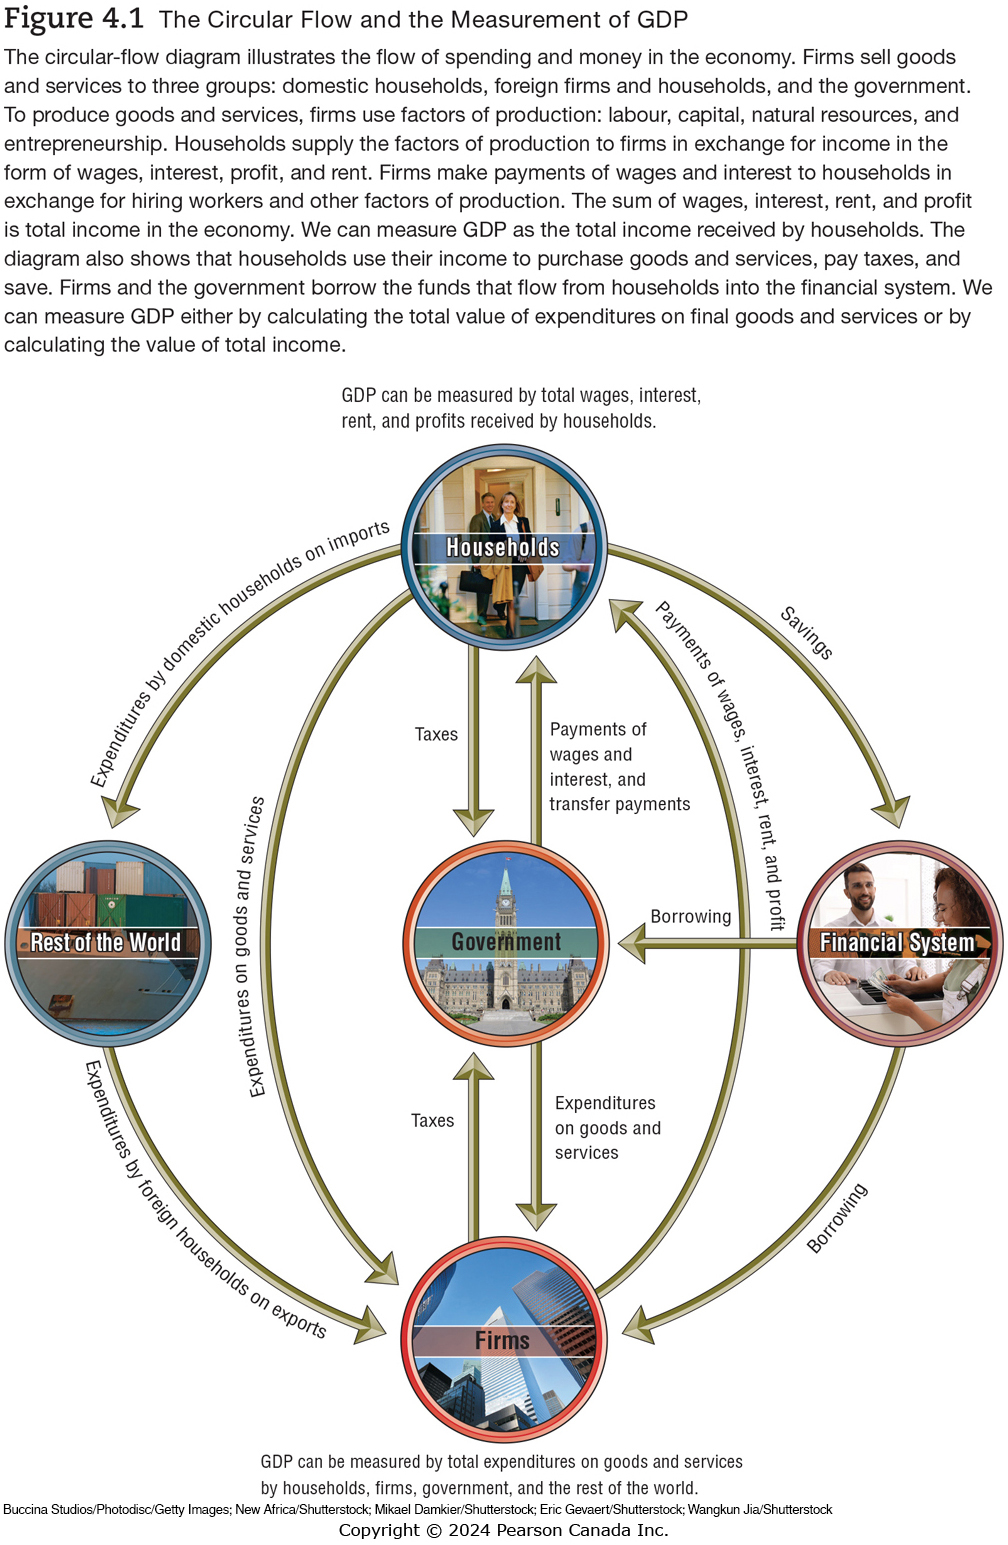
\includegraphics[width=0.43\linewidth]{Fig04-001}.
%\end{frame}







\begin{frame}{Why These Concepts Matter for GDP}
\transfade
\begin{itemize}[<+->]
  \item GDP is our main measure of the \textbf{size of the economy}.
  \item Over time:
  \begin{itemize}[<+->]
    \item Short-run \alert{business cycles} show up as ups and downs in real GDP.
    \item Long-run \alert{economic growth} shows up as an upward trend in real GDP.
  \end{itemize}
  \item Inflation affects \textbf{nominal} GDP, so we must distinguish it from \textbf{real} GDP.
\end{itemize}
\end{frame}

% ============================================================
\section{4.1 Gross Domestic Product Measures Total Production}
% ============================================================

\begin{frame}{4.1 Learning Objective}
\transfade
\begin{block}{Goal}
Explain how total production is measured.
\end{block}
\begin{itemize}[<+->]
  \item The most common measure of overall economic activity is \textbf{gross domestic product (GDP)}.
  \item \textbf{Definition:}  
  Gross domestic product (GDP) is the \alert{market value of all final goods and services produced in a country during a period of time}, typically one year.
  \item We will unpack each phrase in this definition:
  \begin{itemize}[<+->]
    \item ``market value''
    \item ``final goods and services''
    \item ``produced in a country''
    \item ``during a period of time''
  \end{itemize}
\end{itemize}
\end{frame}

\begin{frame}{``Market Value''}
\transfade
\begin{itemize}[<+->]
  \item We produce many different goods and services:
  \begin{itemize}[<+->]
    \item cars, melons, haircuts, concerts, streaming services, etc.
  \end{itemize}
  \item We cannot simply add \emph{physical quantities} (e.g., 100 cars + 500 haircuts).
  \item We need a \alert{common unit of measurement}.
  \item The most practical common unit is \textbf{money}.
  \item We value each good or service at its \alert{market price}.  
  This gives us the \textbf{market value} of production.
\end{itemize}
\end{frame}

\begin{frame}{Final Goods and Services (1 of 2)}
\transfade
\begin{itemize}[<+->]
  \item GDP counts the market value of all \textbf{final} goods and services.
  \item A \textbf{final good or service} is purchased by a \alert{final user}.
  \item These are the items included directly in GDP.
  \item \textbf{Intermediate goods and services} are inputs into other goods and services.
  \begin{itemize}[<+->]
    \item Example: a tire installed on a new truck, flour used in bread, steel used in cars.
  \end{itemize}
\end{itemize}
\end{frame}

\begin{frame}{Final Goods and Services (2 of 2): Avoiding Double Counting}
\transfade
\begin{itemize}[<+->]
  \item If we counted intermediate goods and also counted the final goods that use them, we would \alert{double count}.
  \item Example:
  \begin{itemize}[<+->]
    \item A store buys ice cream from a manufacturer.
    \item Later, the store sells that same ice cream to consumers.
    \item If we counted both the store's purchase and the consumers' purchase in GDP, the value of the ice cream would be counted twice.
  \end{itemize}
  \item To avoid this, we count \textbf{only the final sale} to the consumer.
\end{itemize}
\end{frame}

\begin{frame}{GDP and Where Production Occurs}
\transfade
\begin{itemize}[<+->]
  \item GDP measures production within a \alert{country's borders}.
  \begin{itemize}[<+->]
    \item It includes production by a Canadian firm or a foreign firm, as long as it takes place in Canada.
    \item It excludes production that takes place outside Canada, even if it is done by Canadian-owned firms.
  \end{itemize}
  \item Example:
  \begin{itemize}[<+->]
    \item A Japanese-owned auto plant in Ontario \(\Rightarrow\) included in Canadian GDP.
    \item A Canadian mining company producing in Chile \(\Rightarrow\) not included in Canadian GDP.
  \end{itemize}
\end{itemize}
\end{frame}

\begin{frame}{``During a Period of Time''}
\transfade
\begin{itemize}[<+->]
  \item GDP is measured for a specific period:
  \begin{itemize}[<+->]
    \item usually a \textbf{year}, sometimes a \textbf{quarter} (three months).
  \end{itemize}
  \item We count goods and services \alert{produced during} that time.
  \item This avoids double counting across years.
  \item Example:
  \begin{itemize}[<+->]
    \item A textbook produced and sold new in 2022 is part of 2022 GDP.
    \item The same textbook re-sold used in 2023 does \textbf{not} count again in 2023 GDP.
    \item Used goods were already counted when they were first produced.
  \end{itemize}
\end{itemize}
\end{frame}

\begin{frame}{Production and Income: Two Sides of the Same Coin}
\transfade
\begin{itemize}[<+->]
  \item There are two main ways to measure total economic activity:
  \begin{itemize}[<+->]
    \item The value of \textbf{total production}.
    \item The value of \textbf{total income}.
  \end{itemize}
  \item When something is produced and sold, it generates \alert{income} for someone:
  \begin{itemize}[<+->]
    \item workers receive wages,
    \item owners of capital receive profit or interest,
    \item landowners receive rent, etc.
  \end{itemize}
  \item Therefore, in principle:  
  \[
    \text{Total Production} = \text{Total Income}.
  \]
\end{itemize}
\end{frame}

% ------------------------------------------------------------
% Circular Flow & GDP
% ------------------------------------------------------------

\begin{frame}{Figure 4.1 -- The Circular Flow and GDP (1 of 4)}
\transfade
\begin{itemize}[<+->]
  \item Start with a simple model of households and firms.
  \item Households:
  \begin{itemize}[<+->]
    \item Supply factors of production (labour, capital, natural resources, entrepreneurship).
    \item Receive income in return (wages, interest, profit, rent).
  \end{itemize}
  \item Firms:
  \begin{itemize}[<+->]
    \item Use these inputs to produce goods and services.
    \item Sell output to households.
  \end{itemize}
\end{itemize}
\end{frame}

\begin{frame}{Figure 4.1 -- Circular Flow: Basic Version}
\centering


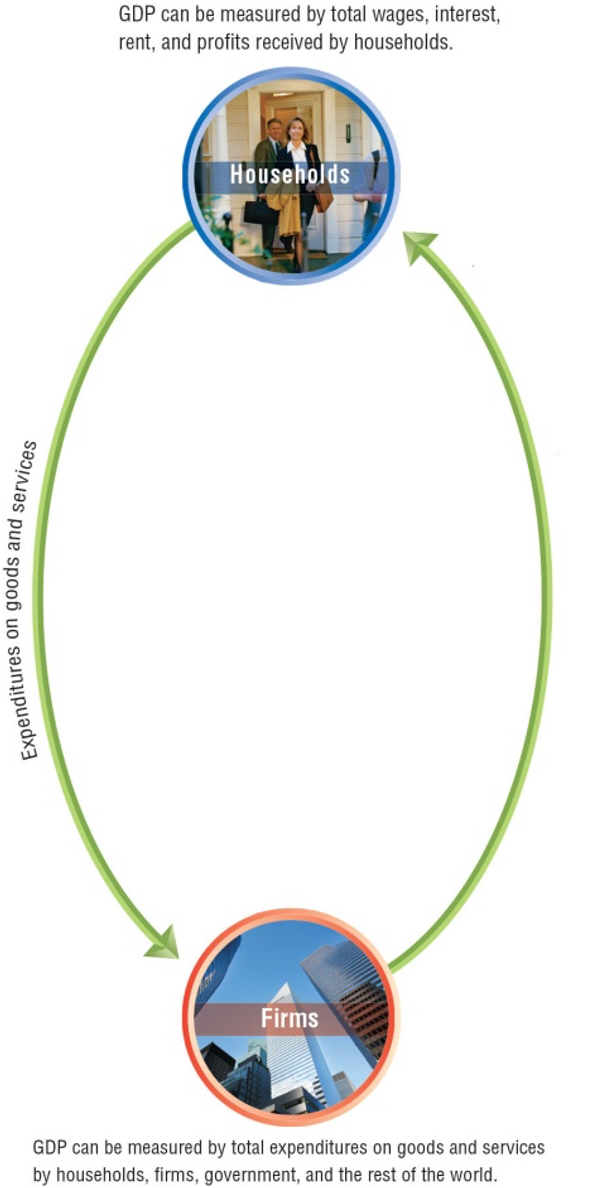
\includegraphics[width=0.25\linewidth]{Fig04-001a}.
\end{frame}

\begin{frame}{Figure 4.1 -- Adding Government (2 of 4)}
\transfade
\begin{itemize}[<+->]
  \item Government collects \textbf{taxes} from households and firms.
  \item Government purchases goods and services from firms (\(G\)).
  \item Government makes \textbf{transfer payments} to households:
  \begin{itemize}[<+->]
    \item e.g., Employment Insurance, Old Age Security.
  \end{itemize}
  \item Transfer payments are \alert{not} payment for current production, so they are \textbf{not directly counted} in GDP.
\end{itemize}
\end{frame}

\begin{frame}{Figure 4.1 -- Adding Government}
\centering


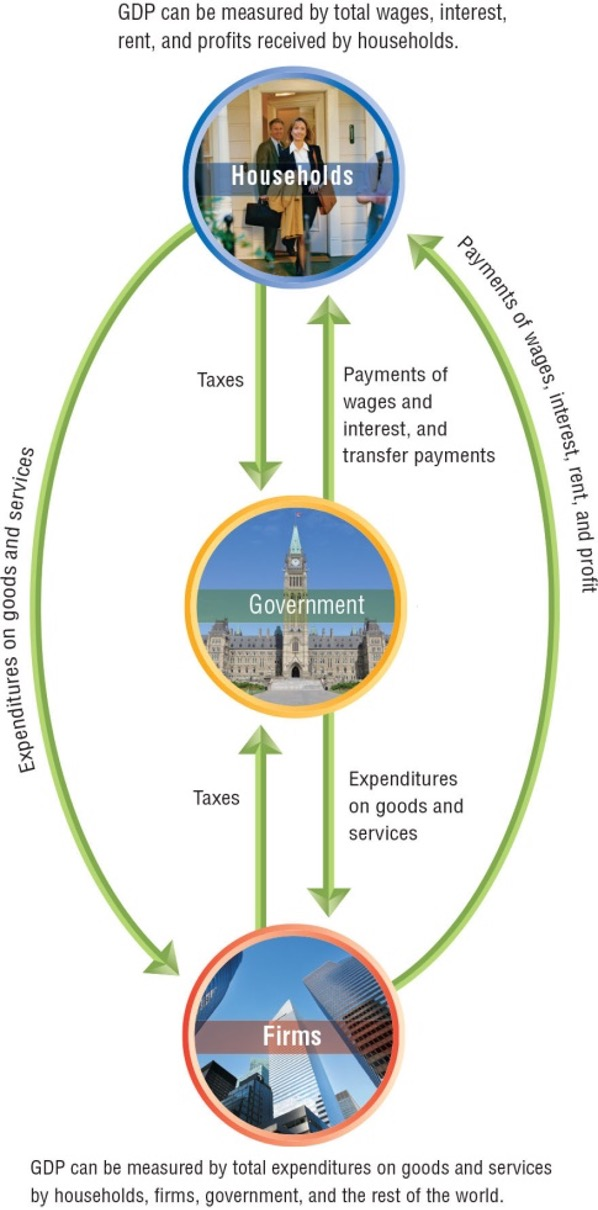
\includegraphics[width=0.25\linewidth]{Fig04-001b}.
\end{frame}

\begin{frame}{Figure 4.1 -- Open Economy: Exports and Imports (3 of 4)}
\transfade
\begin{itemize}[<+->]
  \item Households, firms, and governments interact with the \textbf{rest of the world}.
  \item \textbf{Exports (X):}
  \begin{itemize}[<+->]
    \item Goods and services produced in Canada and sold abroad.
  \end{itemize}
  \item \textbf{Imports (M):}
  \begin{itemize}[<+->]
    \item Goods and services produced abroad and purchased in Canada.
  \end{itemize}
  \item Net exports: \(\text{NX} = X - M\).
\end{itemize}
\end{frame}

\begin{frame}{Figure 4.1 -- Open Economy Flows}
\centering


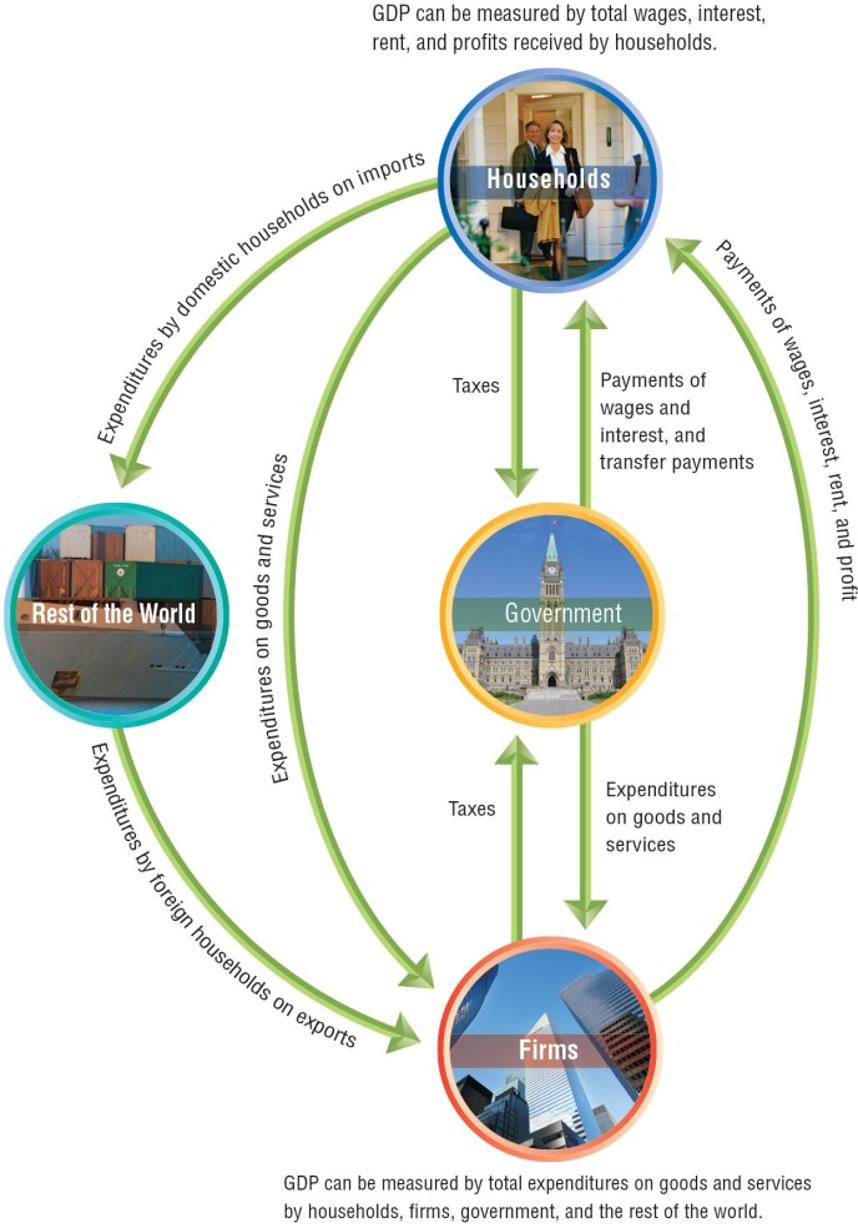
\includegraphics[width=0.35\linewidth]{Fig04-001c}.
\end{frame}

\begin{frame}{Figure 4.1 -- Financial System (4 of 4)}
\transfade
\begin{itemize}[<+->]
  \item Households do not spend all of their income:
  \begin{itemize}[<+->]
    \item Some is saved with banks and other financial institutions.
  \end{itemize}
  \item The \textbf{financial system} channels these savings to:
  \begin{itemize}[<+->]
    \item firms (for investment spending),
    \item governments (for borrowing).
  \end{itemize}
  \item This completes the circular flow of income and spending.
\end{itemize}
\end{frame}

\begin{frame}{Figure 4.1 -- Full Circular Flow }
\centering


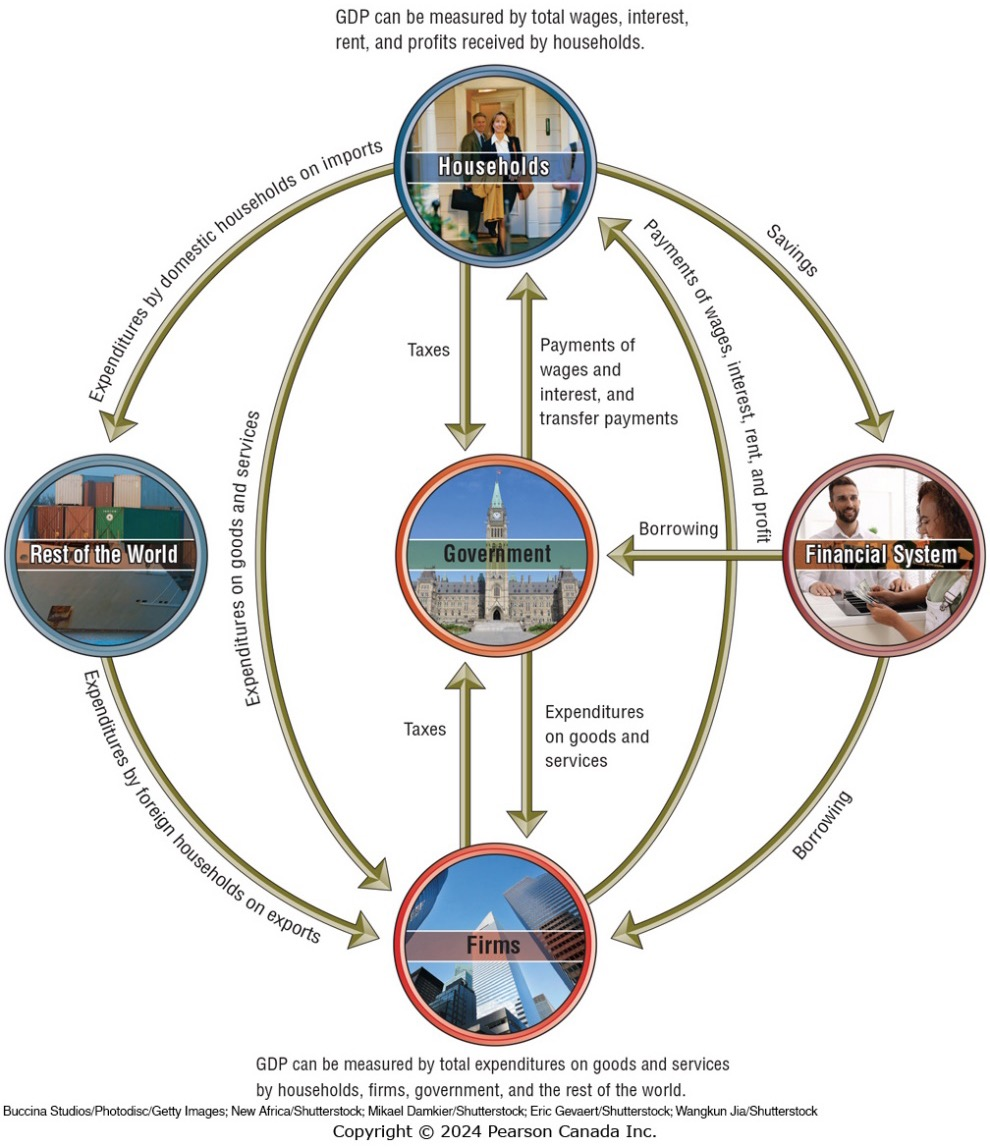
\includegraphics[width=0.445\linewidth]{Fig04-001d}.
\end{frame}

% ------------------------------------------------------------
% Income Approach
% ------------------------------------------------------------

\begin{frame}{Income Approach to Measuring GDP}
\transfade
\begin{itemize}[<+->]
  \item One way Statistics Canada measures GDP is by tracking \textbf{incomes}.
  \item The income approach has \alert{five components}:
  \begin{itemize}[<+->]
    \item Compensation of employees
    \item Gross operating surplus
    \item Gross mixed income
    \item Taxes less subsidies
    \item Statistical discrepancy
  \end{itemize}
\end{itemize}
\end{frame}

\begin{frame}{Compensation of Employees}
\transfade
\begin{itemize}[<+->]
  \item \textbf{Compensation of employees} covers all benefits workers receive from providing their labour.
  \item It is the \alert{single largest} element of GDP in the income approach, about \textbf{50\%} of GDP.
  \item Two components:
  \begin{itemize}[<+->]
    \item \textbf{Wages and salaries:} money paid directly to workers (\(\approx 44\%\) of GDP in 2021).
    \item \textbf{Employers' social contributions:} payments made by employers on behalf of employees to social programs (\(\approx 7\%\) of GDP in 2021).
  \end{itemize}
\end{itemize}
\end{frame}

\begin{frame}{Gross Operating Surplus}
\transfade
\begin{itemize}[<+->]
  \item \textbf{Gross operating surplus} covers payments to owners of the \alert{capital} used by firms and government.
  \item It accounted for about \textbf{27.7\%} of GDP in 2021.
  \item Two elements:
  \begin{itemize}[<+->]
    \item \textbf{Net operating surplus:} payments to owners of capital over and above compensation for capital that wore out (\(\approx 14.2\%\) of GDP in 2021).
    \item \textbf{Capital consumption} (depreciation): payments to owners to cover capital that wore out (\(\approx 13.4\%\) of GDP in 2021).
  \end{itemize}
\end{itemize}
\end{frame}

\begin{frame}{Gross Mixed Income}
\transfade
\begin{itemize}[<+->]
  \item \textbf{Gross mixed income} covers income generated by small businesses for their owners.
  \item It accounted for about \textbf{11.9\%} of GDP.
  \item Two parts:
  \begin{itemize}[<+->]
    \item \textbf{Consumption of fixed capital:} depreciation of capital used by small businesses (\(\approx 3.1\%\) of GDP).
    \item \textbf{Net mixed income:} payment to owners over and above depreciation (\(\approx 8.7\%\) of GDP).
  \end{itemize}
\end{itemize}
\end{frame}

\begin{frame}{Taxes Less Subsidies}
\transfade
\begin{itemize}[<+->]
  \item \textbf{Taxes less subsidies} are payments to government that act like income received by owners of other inputs.
  \item This component accounted for about \textbf{9.4\%} of GDP.
  \item Intuition:
  \begin{itemize}[<+->]
    \item These are part of the value created in production, but they go to government instead of private input owners.
  \end{itemize}
\end{itemize}
\end{frame}

\begin{frame}{Income Approach Summary Table}
\transfade
\small
\begin{tabular}{l c}
\toprule
\textbf{Component} & \textbf{Approximate Share of GDP (2021)} \\
\midrule
Compensation of employees & 50\% \\
\quad Wages and salaries & 44\% \\
\quad Employers' social contributions & 7\% \\
Gross operating surplus & 27.7\% \\
\quad Net operating surplus & 14.2\% \\
\quad Capital consumption & 13.4\% \\
Gross mixed income & 11.9\% \\
\quad Consumption of fixed capital & 3.1\% \\
\quad Net mixed income & 8.7\% \\
Taxes less subsidies & 9.4\% \\
Statistical discrepancy & very small (around 0.0004\%) \\
\bottomrule
\end{tabular}
\end{frame}

% ------------------------------------------------------------
% Expenditure Approach
% ------------------------------------------------------------

\begin{frame}{Expenditure Approach to Measuring GDP}
\transfade
\begin{itemize}[<+->]
  \item Another way to measure GDP is to track \textbf{spending} on final goods and services.
  \item The expenditure approach has \alert{five components} in the national accounts:
  \begin{itemize}[<+->]
    \item Final consumption
    \item Gross fixed capital formation
    \item Investment in inventories
    \item Net exports of goods and services
    \item Statistical discrepancy
  \end{itemize}
\end{itemize}
\end{frame}

\begin{frame}{Final Consumption}
\transfade
\begin{itemize}[<+->]
  \item \textbf{Final consumption:} all domestic purchases of goods and services by their final users.
  \item Includes purchases such as:
  \begin{itemize}[<+->]
    \item clothing,
    \item paper by government,
    \item food purchased by food banks.
  \end{itemize}
  \item Final consumption is about \textbf{77\%} of GDP.
\end{itemize}
\end{frame}

\begin{frame}{Final Consumption by Sector}
\transfade
\small
\begin{itemize}[<+->]
  \item Statistics Canada breaks final consumption into three elements:
\end{itemize}
\begin{tabular}{l c}
\toprule
\textbf{Spender} & \textbf{Share of GDP} \\
\midrule
Households & 54.1\% \\
Government & 21.4\% \\
Not-for-profit organizations & 1.5\% \\
\midrule
\textbf{Total final consumption} & 77.0\% \\
\bottomrule
\end{tabular}
\end{frame}

\begin{frame}{Gross Fixed Capital Formation}
\transfade
\begin{itemize}[<+->]
  \item \textbf{Gross fixed capital formation:} purchases of fixed assets (capital) by firms, governments, and households.
  \item Fixed assets:
  \begin{itemize}[<+->]
    \item provide benefits over a long period,
    \item cannot easily be converted into cash.
    \item Examples: buildings, machinery, equipment, software.
  \end{itemize}
  \item Gross fixed capital formation is about \textbf{23.2\%} of GDP.
\end{itemize}
\end{frame}

\begin{frame}{Gross Fixed Capital Formation by Sector}
\transfade
\small
\begin{tabular}{l c}
\toprule
\textbf{Purchaser} & \textbf{Share of GDP} \\
\midrule
Business & 19.1\% \\
Government & 4.0\% \\
\midrule
\textbf{Total gross fixed capital formation} & 23.2\% \\
\bottomrule
\end{tabular}

\vspace{0.7em}
\begin{itemize}[<+->]
  \item Business investment is crucial for \alert{future productivity growth}.
  \item Government capital spending supports infrastructure, schools, hospitals, etc.
\end{itemize}
\end{frame}

\begin{frame}{Investment in Inventories}
\transfade
\begin{itemize}[<+->]
  \item \textbf{Investment in inventories:} spending on finished products kept on hand to sell later.
  \item If inventories rise, there is \alert{positive} inventory investment.
  \item If inventories fall, inventory investment is \alert{negative}.
  \item Example:
  \begin{itemize}[<+->]
    \item In 2021, inventory investment in Canada was about \(-\$13{,}368\).
    \item Firms were selling more out of inventory than they were adding.
  \end{itemize}
\end{itemize}
\end{frame}

\begin{frame}{Net Exports of Goods and Services}
\transfade
\begin{itemize}[<+->]
  \item \textbf{Net exports (NX)} = exports \(-\) imports.
  \item Exports:
  \begin{itemize}[<+->]
    \item Goods and services produced in Canada and sold to foreign buyers.
  \end{itemize}
  \item Imports:
  \begin{itemize}[<+->]
    \item Goods and services produced abroad and bought by Canadian buyers.
  \end{itemize}
  \item Net exports were about \textbf{2.8\%} of GDP in 2021, and often \alert{negative} for Canada:
  \begin{itemize}[<+->]
    \item Exports: 30.8\% of GDP.
    \item Imports: 30.6\% of GDP.
  \end{itemize}
\end{itemize}
\end{frame}

\begin{frame}{Statistical Discrepancy (Expenditure Side)}
\transfade
\begin{itemize}[<+->]
  \item In practice, the income and expenditure approaches do not match perfectly.
  \item \textbf{Statistical discrepancy:}
  \begin{itemize}[<+->]
    \item An adjustment item that ensures the two approaches yield the same GDP.
    \item Reflects small measurement errors and different estimation techniques.
  \end{itemize}
  \item Statistics Canada:
  \begin{itemize}[<+->]
    \item Takes the difference between income-based and expenditure-based GDP,
    \item Divides it in half,
    \item Adds one half to the lower estimate and subtracts one half from the higher.
  \end{itemize}
\end{itemize}
\end{frame}

\begin{frame}{The Expenditure Approach in Macro Models}
\transfade
\begin{itemize}[<+->]
  \item In macro models, we often use a slightly different breakdown:
  \[
    Y = C + I + G + NX
  \]
  \item \textbf{Consumption (C):}
  \begin{itemize}[<+->]
    \item Final consumption expenditure by households.
  \end{itemize}
  \item \textbf{Investment (I):}
  \begin{itemize}[<+->]
    \item Business spending on fixed capital and inventories.
  \end{itemize}
  \item \textbf{Government spending (G):}
  \begin{itemize}[<+->]
    \item Government fixed capital formation and final consumption.
  \end{itemize}
  \item \textbf{Net exports (NX):}
  \begin{itemize}[<+->]
    \item Exports minus imports.
  \end{itemize}
\end{itemize}
\end{frame}

\begin{frame}{Components of GDP: Big Picture}
\transfade
\begin{itemize}[<+->]
  \item In Canada:
  \begin{itemize}[<+->]
    \item \textbf{Consumption} is the largest component of GDP.
    \item Within consumption, \textbf{services} are the largest subcomponent (almost half of GDP).
    \item \textbf{Investment} and \textbf{government spending} are smaller, but crucial for growth and public services.
    \item \textbf{Net exports} are often slightly negative and reduce GDP.
  \end{itemize}
\end{itemize}
\end{frame}

\begin{frame}{Components of GDP }
\centering


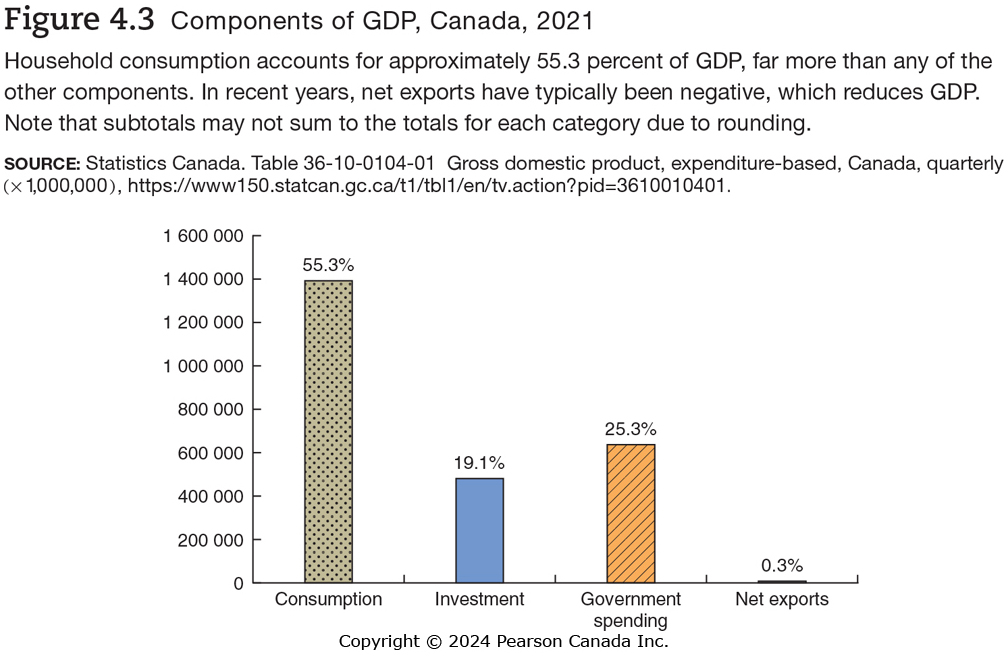
\includegraphics[width=0.78\linewidth]{Fig04-003}.
\end{frame}

\begin{frame}{Table 4.1 -- Calculating Value Added (Placeholder)}
\centering


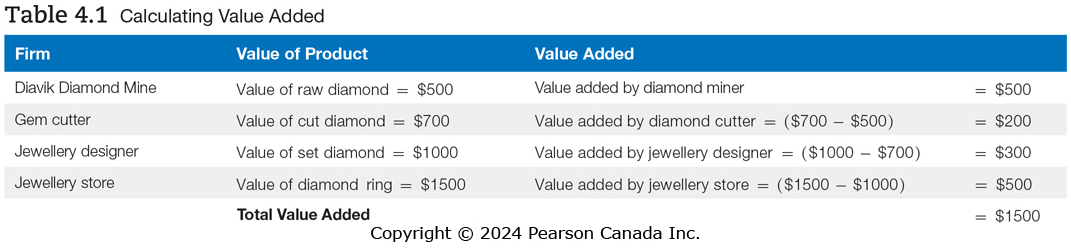
\includegraphics[width=1\linewidth]{Tab04-0001}.
\end{frame}

% ============================================================
\section{4.2 Does GDP Measure What We Want It to Measure?}
% ============================================================

\begin{frame}{4.2 Learning Objective}
\transfade 
\begin{block}{Goal}
Discuss whether GDP is a good measure of well-being.
\end{block}
\begin{itemize}[<+->]
  \item GDP is a useful measure of total output.
  \item Many people interpret GDP as a measure of citizens' \alert{economic well-being}.
  \item However, GDP has shortcomings:
  \begin{itemize}[<+->]
    \item as a measure of \textbf{total production},
    \item as a measure of \textbf{well-being}.
  \end{itemize}
\end{itemize}
\end{frame}

\begin{frame}{Shortcomings of GDP as a Measure of Total Production}
\transfade
\begin{itemize}[<+->]
  \item Two important types of production are omitted:
  \begin{itemize}[<+->]
    \item \textbf{Household production}
    \item \textbf{Informal (shadow) economy}
  \end{itemize}
\end{itemize}
\end{frame}

\begin{frame}{Household Production}
\transfade
\begin{itemize}[<+->]
  \item Household production includes unpaid activities such as:
  \begin{itemize}[<+->]
    \item childcare,
    \item cleaning,
    \item cooking,
    \item home repairs.
  \end{itemize}
  \item If these tasks were performed by someone outside the household and paid for, they \textbf{would} be counted in GDP.
  \item Because they are unpaid, they are \alert{omitted} from GDP, even though they create real value.
\end{itemize}
\end{frame}

\begin{frame}{Informal Economy}
\transfade
\begin{itemize}[<+->]
  \item The \textbf{informal economy} (or shadow economy) consists of:
  \begin{itemize}[<+->]
    \item Legal activities not reported to the government (to avoid taxes or regulations).
    \item Illegal activities (e.g., some black-market transactions).
  \end{itemize}
  \item These transactions create value and income but are not captured in official GDP statistics.
  \item Estimates suggest the Canadian shadow economy is about \textbf{13\%} of officially measured GDP, and higher in many low-income countries.
\end{itemize}
\end{frame}

\begin{frame}{How Serious Are These Omissions?}
\transfade
\begin{itemize}[<+->]
  \item For \textbf{year-to-year comparisons}:
  \begin{itemize}[<+->]
    \item Household production and the informal economy are likely roughly constant as a share of GDP.
    \item So GDP growth is still a reasonable measure of growth in total production.
  \end{itemize}
  \item Over \textbf{longer periods}, the omissions can matter more.
  \item Example:
  \begin{itemize}[<+->]
    \item As more women enter the paid labour force, tasks once done at home (childcare, cooking) are replaced by market activities.
    \item GDP rises, but part of the increase reflects a \alert{shift from home to market}, not entirely new production.
  \end{itemize}
\end{itemize}
\end{frame}

\begin{frame}{Shortcomings of GDP as a Measure of Well-Being}
\transfade
\begin{itemize}[<+->]
  \item GDP per person (\textbf{GDP per capita}) is often used as a measure of the \alert{standard of living}.
  \item But even if GDP accurately measures total production, it does not capture:
  \begin{itemize}[<+->]
    \item the value of \textbf{leisure},
    \item \textbf{pollution} and other negative by-products of production,
    \item \textbf{crime} and other social problems,
    \item the \textbf{distribution of income}.
  \end{itemize}
\end{itemize}
\end{frame}

\begin{frame}{Example: Crime and Well-Being}
\transfade
\begin{itemize}[<+->]
  \item Suppose crime falls significantly.
  \item Less spending is needed on:
  \begin{itemize}[<+->]
    \item police,
    \item prisons,
    \item private security.
  \end{itemize}
  \item GDP might \alert{fall} because some spending drops.
  \item But economic well-being clearly \alert{improves}.
  \item Conclusion: higher GDP is not the only indicator of better lives.
\end{itemize}
\end{frame}

\begin{frame}{GDP and Happiness}
\transfade
\begin{itemize}[<+->]
  \item GDP was not designed to measure happiness or life satisfaction.
  \item Yet, when we compare countries:
  \begin{itemize}[<+->]
    \item Higher GDP per person is often associated with higher measures of well-being (such as broader quality-of-life indices).
    \item Very low GDP per person is almost always associated with low well-being.
  \end{itemize}
  \item So:
  \begin{itemize}[<+->]
    \item GDP is an \alert{imperfect} but \textbf{useful} indicator of economic well-being.
  \end{itemize}
\end{itemize}
\end{frame}

\begin{frame}{Better Life Index vs.\ GDP }
\centering


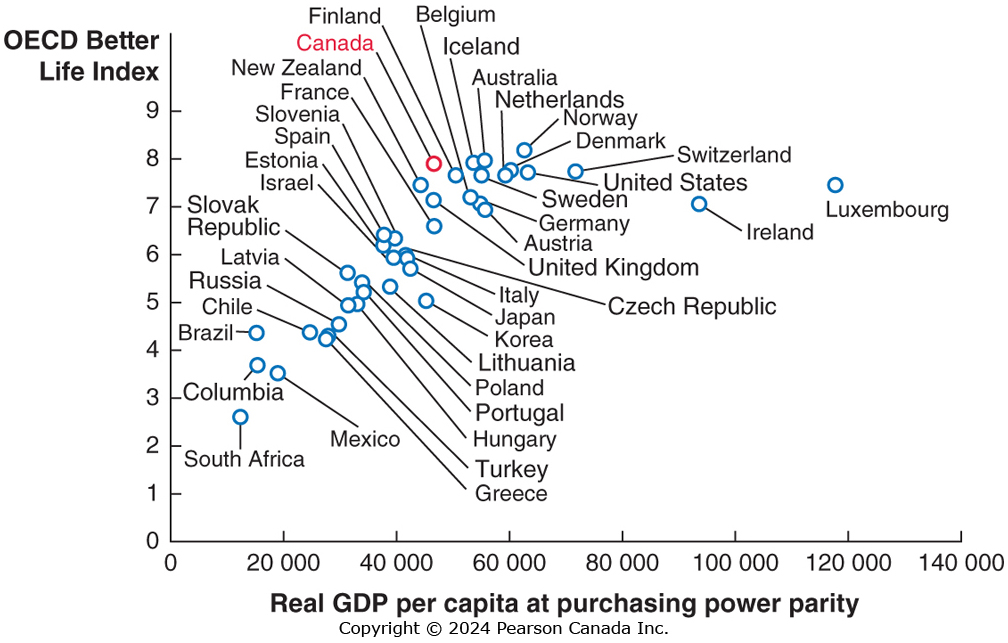
\includegraphics[width=0.74\linewidth]{UnFig04-002}.
\end{frame}

% ============================================================
\section{4.3 Real GDP versus Nominal GDP}
% ============================================================

\begin{frame}{4.3 Learning Objective}
\transfade
\begin{block}{Goal}
Discuss the difference between real GDP and nominal GDP.
\end{block}
\begin{itemize}[<+->]
  \item GDP is measured in dollar terms (market value).
  \item When we compare GDP over time, prices usually \alert{change}.
  \item We must separate:
  \begin{itemize}[<+->]
    \item changes in \textbf{quantities},
    \item changes in \textbf{prices}.
  \end{itemize}
\end{itemize}
\end{frame}

\begin{frame}{Nominal GDP vs.\ Real GDP}
\transfade
\begin{itemize}[<+->]
  \item \textbf{Nominal GDP:}
  \begin{itemize}[<+->]
    \item Value of final goods and services \alert{evaluated at current-year prices}.
  \end{itemize}
  \item \textbf{Real GDP:}
  \begin{itemize}[<+->]
    \item Value of final goods and services \alert{evaluated at base-year prices}.
  \end{itemize}
  \item The base year is arbitrary; in current Canadian data the standard base year is \textbf{2012}.
  \item Real GDP removes the effect of changing prices, allowing us to focus on changes in \textbf{quantities produced}.
\end{itemize}
\end{frame}

\begin{frame}{Calculating Real GDP: Example (1 of 2)}
\transfade
\begin{itemize}[<+->]
  \item Suppose we have three goods, produced in 2012 and 2023.
  \item The table in the slides shows output and prices in 2012 and 2023.
  \item To calculate real GDP in 2023 using 2012 as the base year:
  \begin{itemize}[<+->]
    \item Multiply 2023 quantities by \textbf{2012 prices}, then add up.
    \item The example yields:  
    \[
      \text{Real GDP}_{2023} = 4000 + 880 + 1800 = 6680.
    \]
  \end{itemize}
\end{itemize}
\end{frame}

\begin{frame}{Calculating Real GDP: Example (2 of 2)}
\transfade
\begin{itemize}[<+->]
  \item If we instead valued 2023 output at \textbf{2023 prices}, we would get:
  \[
    \text{Nominal GDP}_{2023} = 7800.
  \]
  \item Because most prices rose from 2012 to 2023, nominal GDP is larger than real GDP.
  \item This highlights why we use \alert{real GDP} to avoid exaggerating growth when prices rise.
\end{itemize}
\end{frame}

\begin{frame}{Figure 4.4 -- Nominal GDP and Real GDP (Diagram Placeholder)}
\centering


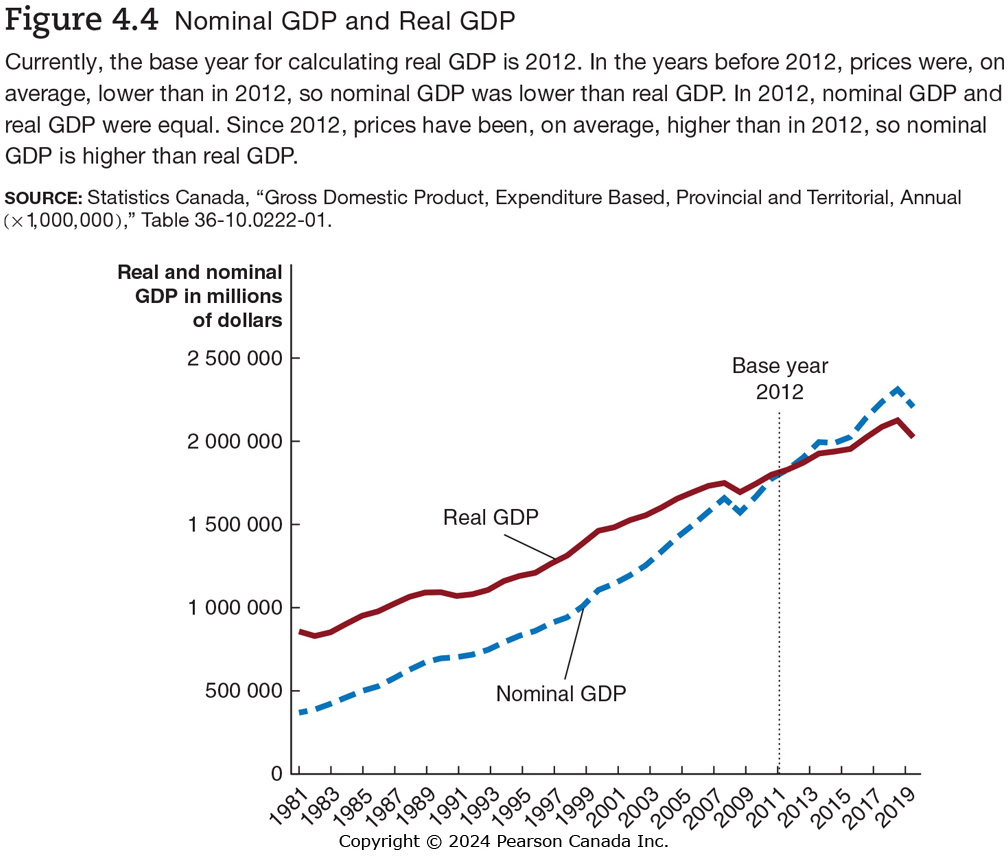
\includegraphics[width=0.56\linewidth]{Fig04-004}.
\end{frame}

\begin{frame}{Interpreting Real GDP}
\transfade
\begin{itemize}[<+->]
  \item In the base year, real and nominal GDP are \textbf{equal}.
  \item After the base year:
  \begin{itemize}[<+->]
    \item If prices in general rise, nominal GDP will grow \alert{faster} than real GDP.
    \item If prices fall, nominal GDP will grow \alert{slower} than real GDP.
  \end{itemize}
  \item Growth rates reported in the media usually refer to \textbf{growth in real GDP}.
\end{itemize}
\end{frame}

\begin{frame}{Improving Real GDP: Chain-Weighted Prices}
\transfade
\begin{itemize}[<+->]
  \item One issue with a fixed base year:
  \begin{itemize}[<+->]
    \item \textbf{Relative prices} change over time.
    \item Using old base-year prices can distort real GDP as we move further away from the base year.
  \end{itemize}
  \item To reduce this distortion, Statistics Canada uses \textbf{chain-weighted} prices:
  \begin{itemize}[<+->]
    \item Uses previous-year prices to adjust current-year production.
    \item This better reflects the changing structure of the economy.
  \end{itemize}
\end{itemize}
\end{frame}

% ------------------------------------------------------------
% GDP Deflator
% ------------------------------------------------------------

\begin{frame}{The GDP Deflator}
\transfade
\begin{itemize}[<+->]
  \item Policymakers care about the \textbf{price level}: the average price of goods and services in the economy.
  \item Stable prices help households and firms plan for the future.
  \item One measure of the price level is the \textbf{GDP deflator}, defined as:
  \[
    \text{GDP Deflator} = \frac{\text{Nominal GDP}}{\text{Real GDP}} \times 100.
  \]
  \item In the base year, nominal and real GDP are equal, so the GDP deflator is \textbf{100}.
\end{itemize}
\end{frame}

\begin{frame}{Calculating the GDP Deflator: Example}
\transfade
\begin{itemize}[<+->]
  \item Suppose the GDP deflator increased from 108.8 to 109.0 between two years.
  \item The inflation rate based on the GDP deflator is:
  \[
    \frac{109.0 - 108.8}{108.8} \times 100 \approx 0.2\%.
  \]
  \item We say the \textbf{price level} rose by about 0.2\% between those years.
\end{itemize}
\end{frame}



% ============================================================
\section{4.4 Other Measures of Total Production and Income}
% ============================================================

\begin{frame}{Other Measures of Total Production and Income}
\transfade
\begin{itemize}[<+->]
  \item GDP is the most common measure, but national accounts also construct:
  \begin{itemize}[<+->]
    \item Gross national income (GNI),
    \item National income,
    \item Personal income,
    \item Disposable personal income.
  \end{itemize}
  \item These measures adjust for:
  \begin{itemize}[<+->]
    \item income flows across borders,
    \item depreciation of capital,
    \item taxes and transfers to households.
  \end{itemize}
  \item They are useful when we study \textbf{household budgets} and \textbf{long-run income dynamics}.
\end{itemize}
\end{frame}

% ============================================================
\section*{Chapter Summary}
% ============================================================

\begin{frame}{Summary}
\transfade
\begin{itemize}[<+->]
  \item \textbf{GDP} measures the size of an economy:
  \begin{itemize}[<+->]
    \item as total production \textbf{or} total income.
  \end{itemize}
  \item GDP measures market activity and \textbf{omits} some important things:
  \begin{itemize}[<+->]
    \item household production,
    \item informal economy.
  \end{itemize}
  \item GDP is not intended to be a complete measure of well-being, but higher GDP per person is usually associated with higher material living standards.
  \item \textbf{Real GDP} controls for inflation; \textbf{nominal GDP} does not.
  \item The \textbf{GDP deflator} is a measure of the overall price level.
  \item National accounts also provide other measures of total production and income for more detailed analysis.
\end{itemize}
\end{frame}

\begin{frame}
\centering
\Huge \textbf{Thank you!}
\end{frame}

\end{document}
